\documentclass[eng,openany]{mgr}
\usepackage{listings}
\usepackage[english]{babel}
\usepackage{graphicx}
\usepackage{hyperref}
\usepackage{tabularx,colortbl} 
\usepackage{rotating}
\usepackage[utf8]{inputenc} 
\setlength\parindent{24pt}
\usepackage[parfill]{parskip}
\usepackage[table,kernelfbox,hyperref]{xcolor}
\usepackage{fancyhdr}
\usepackage{gauss}
%\usepackage[colorinlistoftodos]{todonotes}

\hypersetup{colorlinks=true}
\hypersetup{xurlbordercolor=red!70!black}
\hypersetup{xlinkbordercolor=blue!70!black}
\hypersetup{linkcolor=blue!60!black}
\hypersetup{urlcolor=red!50!black}
\hypersetup{citecolor=green!30!black}
\rfoot{Page \thepage}
\renewcommand\lstlistlistingname{List of Listings}
\newcommand{\linia}{\rule{\linewidth}{0.4mm}}

\definecolor{listlightgray}{gray}{0.93}

\newcommand{\lstsetmylst} {
\lstset{frame = tb,
breaklines=true,
framerule = 0.25pt,
float,
fontadjust,
backgroundcolor={\color{listlightgray}},
basicstyle = {\ttfamily\footnotesize},
identifierstyle = {\ttfamily},
stringstyle = {\ttfamily},
showstringspaces = false,
showtabs = false,
numbers = left,
numbersep = 6pt,
tabsize = 4,
language=C,
floatplacement=!h
}
}

\newcommand{\lstsetatc} {
\lstset{frame = tb,
breaklines=true,
framerule = 0.25pt,
float,
fontadjust,
backgroundcolor={\color{listlightgray}},
basicstyle = {\ttfamily\footnotesize},
keywordstyle = {\ttfamily\color{listkeyword}\textbf},
identifierstyle = {\ttfamily},
commentstyle = {\ttfamily\color{listcomment}\textit},
stringstyle = {\ttfamily},
showstringspaces = false,
showtabs = false,
numbers = left,
numbersep = 6pt,
numberstyle={\ttfamily\color{listnumbers}},
tabsize = 4,
language=C,
floatplacement=!h
}
}

\newcommand{\lstsetatbashnum} {
\lstset{frame = tb,
breaklines=true,
framerule = 0.25pt,
aboveskip=2ex,
float,
fontadjust,
backgroundcolor={\color{listlightgray}},
basicstyle = {\ttfamily\footnotesize},
keywordstyle = {\ttfamily\color{listkeyword}\textbf},
identifierstyle = {\ttfamily},
commentstyle = {\ttfamily\color{listcomment}\textit},
stringstyle = {\ttfamily},
showstringspaces = false,
showtabs = false,
numbers = left,
numbersep = 6pt,
numberstyle={\ttfamily\color{listnumbers}},
tabsize = 4,
language=bash,
floatplacement=!h
}
}
\lstsetmylst
\author{Jaroslaw M. Szumega}
\title{}
\engtitle{}
\supervisor{Rafal Zdunek, D.Sc, K-4/W4}
\field{Electronics}
\specialisation{Advanced Applied Electronics}
\date{15.05.2017}
\begin{document}
\selectlanguage{english}
\maketitle
\tableofcontents
\newpage

\chapter{Solution to the given problems}
\begin{figure}[h]
\centering
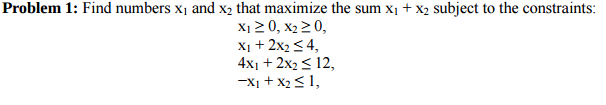
\includegraphics[width=0.7\linewidth]{screenshot001}
\label{fig:screenshot001}
\end{figure}
\begin{figure}[h]
\centering
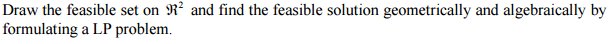
\includegraphics[width=0.7\linewidth]{screenshot002}
\label{fig:screenshot002}
\end{figure}

The given formulas should be rewritten in the matrix form, that will formulate the LP problem to be solved by simplex.


\[
A =
\begin{bmatrix}
1 & 2 \\
4 & 2\\
-1 & 1 
\end{bmatrix}
\]
,
\[
b =
\begin{bmatrix}
4 \\ 12\\  1
\end{bmatrix}
\],
\[
C^T =
\begin{bmatrix}
-1 & 1\\
\end{bmatrix}
\]

At first the computations using coded simplex as well as linprog will be presented:
\begin{lstlisting}
Coded Simplex
x =

2.66667
0.66667

Elapsed time is 0.0161548 seconds.
Linprog
x_lin =

2.66667
0.66667

Elapsed time is 0.00569296 seconds.
\end{lstlisting}

\newpage
Then we will formulate the simplex tableau and calculate the solution step by step (as pointed out in the task's description).
\begin{figure}[h]
\centering
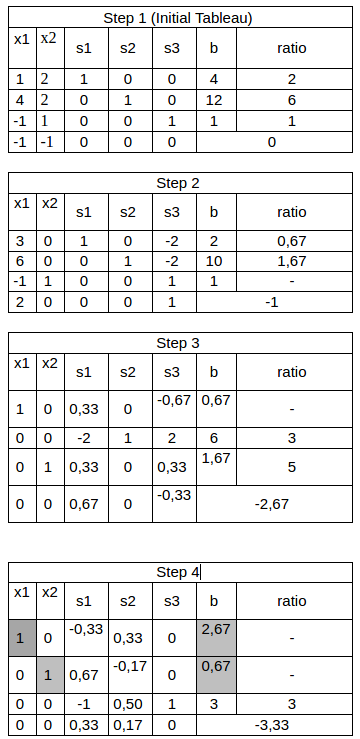
\includegraphics[width=0.3\linewidth]{screenshot004}
\caption{The simplex steps.}
\label{fig:screenshot004}
\end{figure}


The possible solution can be expressed in the graphical form:
\begin{figure}[h]
\centering
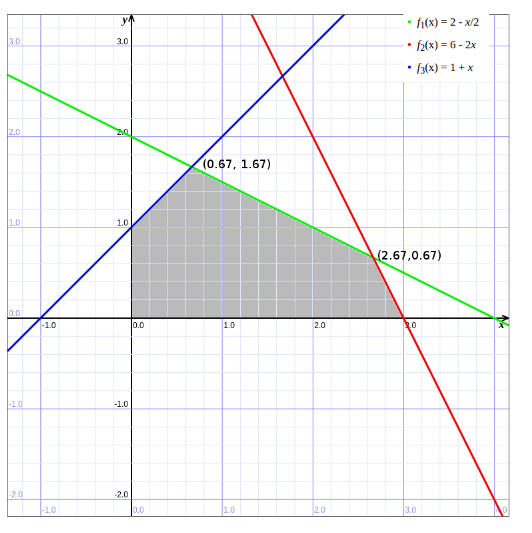
\includegraphics[width=0.4\linewidth]{screenshot003}
\caption{Solution according to x1 and x2 (horizontal and vertical axis)}
\label{fig:screenshot003}
\end{figure}

As it can be noticed, all three methods gave the same solution. Of course, the preparation in case of maximization problem were done -- we used the cost vector with its negative values.
\newpage
\begin{figure}[h]
\centering
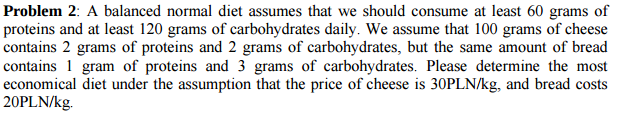
\includegraphics[width=0.7\linewidth]{screenshot005}
\label{fig:screenshot005}
\end{figure}

Basing on the task content, we can write the following formulas:\\
\begin{equation*}
x_1 \geq 0, x_2\geq 0\\
\end{equation*}
\begin{equation*}
2x_1 + x_2 \geq 60\\
\end{equation*}
\begin{equation*}
2x_1 + 3x_2 \geq 120\\
\end{equation*}
\begin{equation*}
min\{30x_1+20x_2\}\\
\end{equation*}


Problem rewritten in the matrix form:

\[
A =
\begin{bmatrix}
2 & 1 \\
2 & 3
\end{bmatrix}
\]
,
\[
b =
\begin{bmatrix}
60 \\ 120
\end{bmatrix}
\],
\[
C^T =
\begin{bmatrix}
30 & 20\\
\end{bmatrix}
\]
Graphical representation:
\begin{figure}[h]
	\centering
	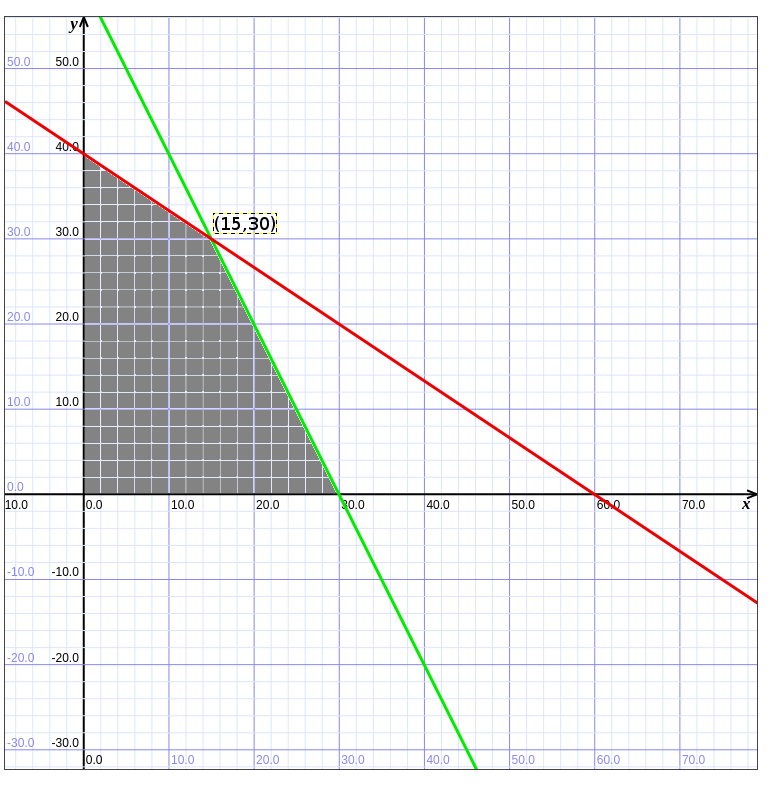
\includegraphics[width=0.5\linewidth]{screenshot006}
	\caption{Graphical representation of functions for economic diet.}
	\label{fig:screenshot006}
\end{figure}

\newpage
\begin{figure}[h]
\centering
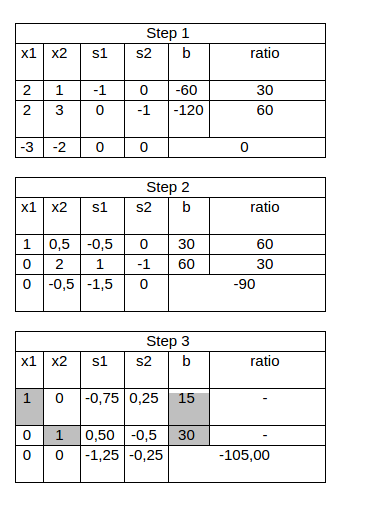
\includegraphics[width=0.4\linewidth]{screenshot007}
\caption{Step by step simplex.}
\label{fig:screenshot007}
\end{figure}

And results of the numerical computations in Octave:

\begin{lstlisting}
Coded Simplex
x =

1.50000
0.50000

Elapsed time is 0.0349259 seconds.


Linprog
x_lin =

1.50000
0.50000

Elapsed time is 0.047415 seconds.
\end{lstlisting}

\newpage
\begin{figure}[h]
\centering
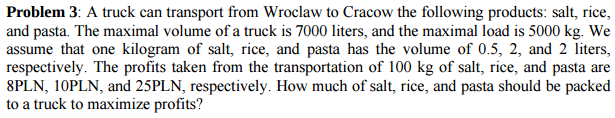
\includegraphics[width=0.7\linewidth]{screenshot008}
\label{fig:screenshot008}
\end{figure}
Basing on the task content, we can write the following formulas:\\
\begin{equation*}
x_1 \geq 0, x_2\geq 0, x_3\geq 0\\
\end{equation*}
\begin{equation*}
0.5x_1 + 2x_2 + 2x_3 \leq 7000\\
\end{equation*}
\begin{equation*}
x_1 + x_2 + x_3 \leq 5000\\
\end{equation*}
\begin{equation*}
max\{0.08x_1+0.1x_2+0.25x_3\}\\
\end{equation*}


Problem rewritten in the matrix form:

\[
A =
\begin{bmatrix}
1/2 & 2 & 2 \\
1 & 1 & 1\\
\end{bmatrix}
\]
,
\[
b =
\begin{bmatrix}
7000 \\ 5000
\end{bmatrix}
\],
\[
C^T =
\begin{bmatrix}
0.08 & 0.1 & 0.25
\end{bmatrix}
\]

\begin{lstlisting}
Coded Simplex x =
2000
0
3000
Elapsed time is 0.0035789 seconds.

Linprog x_lin =
2000
0
3000
Elapsed time is 0.00641394 seconds.
\end{lstlisting}

\begin{figure}[h]
\centering
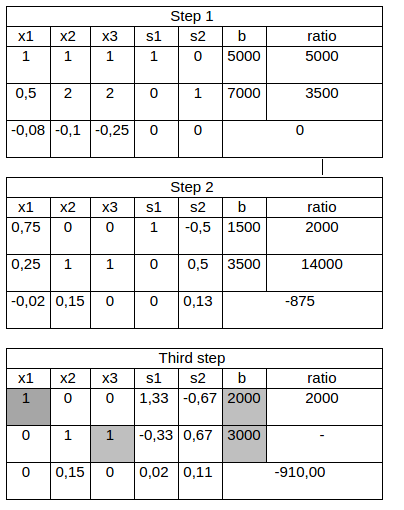
\includegraphics[width=0.3\linewidth]{screenshot009}
\caption{Simplex steps.}
\label{fig:screenshot009}
\end{figure}

\newpage
\begin{figure}[h]
\centering
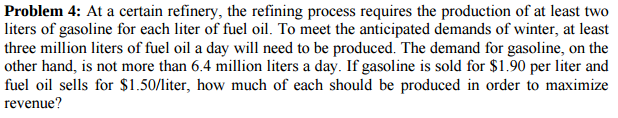
\includegraphics[width=0.7\linewidth]{screenshot010}
\label{fig:screenshot010}
\end{figure}
Basing on the task content, we can write the following formulas:\\
\begin{equation*}
x_1 \geq 0, x_2\geq 0\\
\end{equation*}
\begin{equation*}
-0.5x_1 + x_2 \geq 0\\
\end{equation*}
\begin{equation*}
x_1  \leq 6 400 000\\
\end{equation*}
\begin{equation*}
x_2 \geq 3 000 000\\
\end{equation*}
\begin{equation*}
max\{1.90x_1+1.50x_2\}\\
\end{equation*}


Problem rewritten in the matrix form:

\[
A =
\begin{bmatrix}
1/2 & 2 & 2 \\
1 & 1 & 1\\
\end{bmatrix}
\]
,
\[
b =
\begin{bmatrix}
7000 \\ 5000
\end{bmatrix}
\],
\[
C^T =
\begin{bmatrix}
0.08 & 0.1 & 0.25
\end{bmatrix}
\]
\begin{lstlisting}
Coded Simplex
x =
6.4000
3.0000
Elapsed time is 0.00331903 seconds.

Linprog
x_lin =
6.4000
3.0000
Elapsed time is 0.00622606 seconds.
\end{lstlisting}

\begin{figure}[h]
\centering
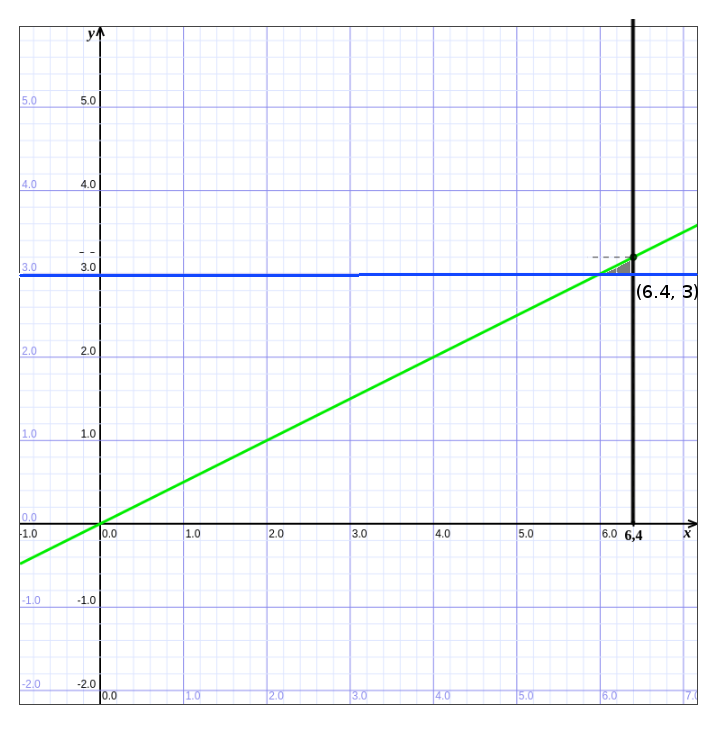
\includegraphics[width=0.4\linewidth]{screenshot011}
\label{fig:screenshot011}
\end{figure}
\newpage
\begin{figure}[h]
\centering
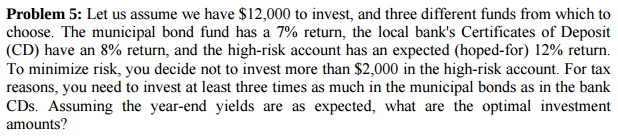
\includegraphics[width=0.7\linewidth]{screenshot012}
\label{fig:screenshot012}
\end{figure}
Basing on the task content, we can write the following formulas:\\
\begin{equation*}
x_1 \geq 0, x_2\geq 0, x_3\geq 0\\
\end{equation*}
\begin{equation*}
x_1 + x_2 + x_3 = 12 000\\
\end{equation*}
\begin{equation*}
x_3 \leq 2 000\\
\end{equation*}
\begin{equation*}
-3x_1-x_2 \leq 0\
\end{equation*}
\begin{equation*}
max\{7x_1 + 8x_2 + 12x_3\}\\
\end{equation*}


Problem rewritten in the matrix form:

\[
A =
\begin{bmatrix}
1 & 1 & 1 \\
0 & 0 & -1\\
-3 & -1 & 0\\
\end{bmatrix}
\]
,
\[
b =
\begin{bmatrix}
12000 \\ 2000 \\ 0
\end{bmatrix}
\],
\[
C^T =
\begin{bmatrix}
7 & 8 & 12
\end{bmatrix}
\]
In this task, only the linprog function returned the feasible solution. In addition only after specifying the additional information such as lowerbond argument.\\
In case of coded simplex the negative numbers were received -- they are not correct, as it is assumed that we accept only nonnegative values.
\begin{lstlisting}
Linprog
x =

7500
2500
2000

Elapsed time is 0.00615597 seconds.
\end{lstlisting}
\newpage

\begin{figure}[h]
\centering
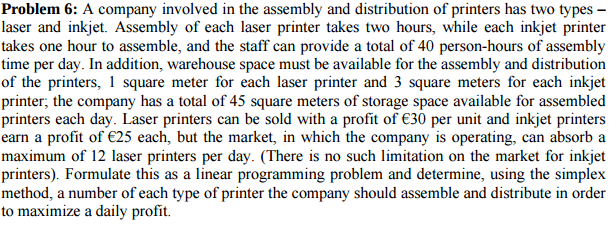
\includegraphics[width=0.7\linewidth]{screenshot013}
\label{fig:screenshot013}
\end{figure}
Basing on the task content, we can write the following formulas:\\
\begin{equation*}
x_1 \geq 0, x_2\geq 0\\
\end{equation*}
\begin{equation*}
2x_1 + x_2 \leq 40\\
\end{equation*}
\begin{equation*}
x_1 + 3x_2 \leq 45\\
\end{equation*}
\begin{equation*}
x_1 \leq 12\
\end{equation*}
\begin{equation*}
max\{30x_1 + 25x_2\}\\
\end{equation*}


Problem rewritten in the matrix form:

\[
A =
\begin{bmatrix}
2 & 1\\
1 & 3\\
1 & 0\\
\end{bmatrix}
\]
,
\[
b =
\begin{bmatrix}
40 \\ 45 \\ 12
\end{bmatrix}
\],
\[
C^T =
\begin{bmatrix}
30 & 25
\end{bmatrix}
\]

\begin{lstlisting}
Coded Simplex
x =
12
11

Elapsed time is 0.00107002 seconds.


Linprog
x_lin =
12
11

Elapsed time is 0.00189614 seconds.
\end{lstlisting}

\begin{figure}[h]
\centering
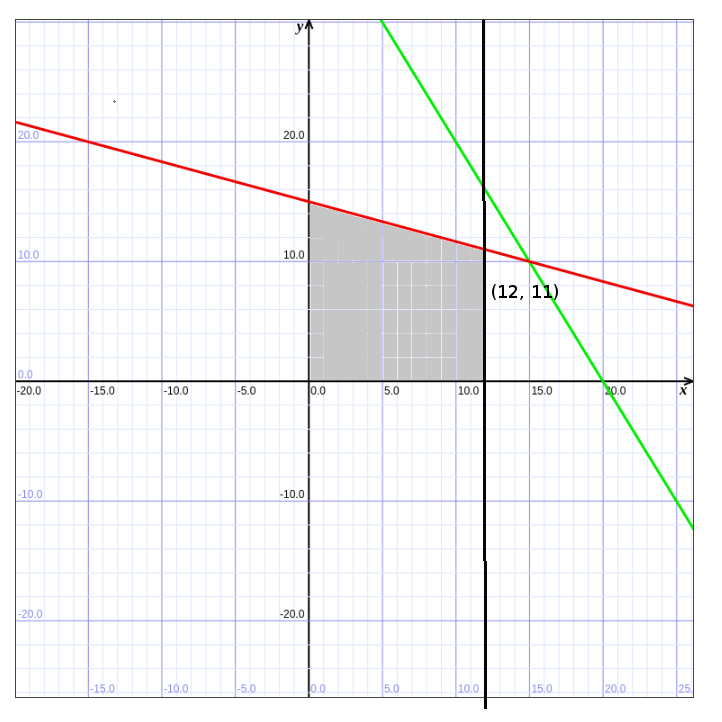
\includegraphics[width=0.5\linewidth]{screenshot014}
\caption{Graphical solution for printers store.}
\label{fig:screenshot014}
\end{figure}

\chapter{Listings of algorithms}
\section{Coded selected algorithms}
Algorithm 1 - Simplex algorithm\\ 
\begin{lstlisting}
function [x] = simplex(A, b, c)

[m,n] = size(A);


#creating initial tableau
diagonal = eye(m);
T = [A diagonal b];
ct = [c zeros(1,m + 1)];
T = [T;ct];

[r, c] = size(T);

#iterating trhough variables - columns
pivot = 0;
for i = 1:c
	#find minimum in the last row
	[val pivot_col] = min(T(r,:));
	
	if val < 0
		pivot_row = findPivot(T, pivot_col);
	else
		x = zeros(n,1);
		for it=1:n
			[piv, spot] = max(T(:,it));
			
			if(T(r,it) == 0)
				x(it,1) = T(spot,c);
			else 
				x(it,1) = 0;
			endif
		endfor
		break;
	endif
	
	
	if pivot_row > 0
		i = pivot_col;
		j = pivot_row;
		T(j,:) = T(j,:)/T(j,i);
		for k = 1: r
			if (k != j)
				T(k,:) = T(k,:) - T(k,i)*T(j,:);
			endif
		endfor
	endif
endfor

endfunction
\end{lstlisting}
\begin{thebibliography}{8}
\addcontentsline{toc}{chapter}{Bibliography}
%\addcontentsline{toc}{section}{Literatura}
\bibitem{bjorck}
\bibitem{zdunek}
Zdunek R., Optimization Methods - lecture slides.
\end{thebibliography}

\end{document}

